% Figure 1: study design (TikZ). Compile with: tectonic Figure1.tex  (or pdflatex Figure1.tex)
% Four stages left to right; one band for the baselines used at every stage. No results.
\documentclass[tikz,border=4pt]{standalone}
\usepackage[T1]{fontenc}
\usepackage{tgheros}
\renewcommand{\familydefault}{\sfdefault}
\hyphenpenalty=10000
\exhyphenpenalty=10000
\usetikzlibrary{arrows.meta,positioning,calc}

\definecolor{ink}{HTML}{0B0B0B}
\definecolor{ink2}{HTML}{52514E}
\definecolor{edge}{HTML}{C3C2B7}
\definecolor{card}{HTML}{F6F5F1}
\definecolor{blue}{HTML}{2A78D6}

\tikzset{
  stage/.style={draw=edge, line width=0.5pt, fill=card, rounded corners=3pt,
                text width=3.35cm, minimum height=2.45cm, align=left, inner sep=6pt, anchor=north},
  head/.style={fill=blue, text=white, rounded corners=3pt, font=\bfseries\small,
               text width=3.35cm, inner xsep=6pt, inner ysep=4pt, text height=1.8ex, text depth=0.5ex,
               align=left, anchor=south},
  flow/.style={-{Stealth[length=5pt]}, line width=0.8pt, draw=ink2},
}

\begin{document}
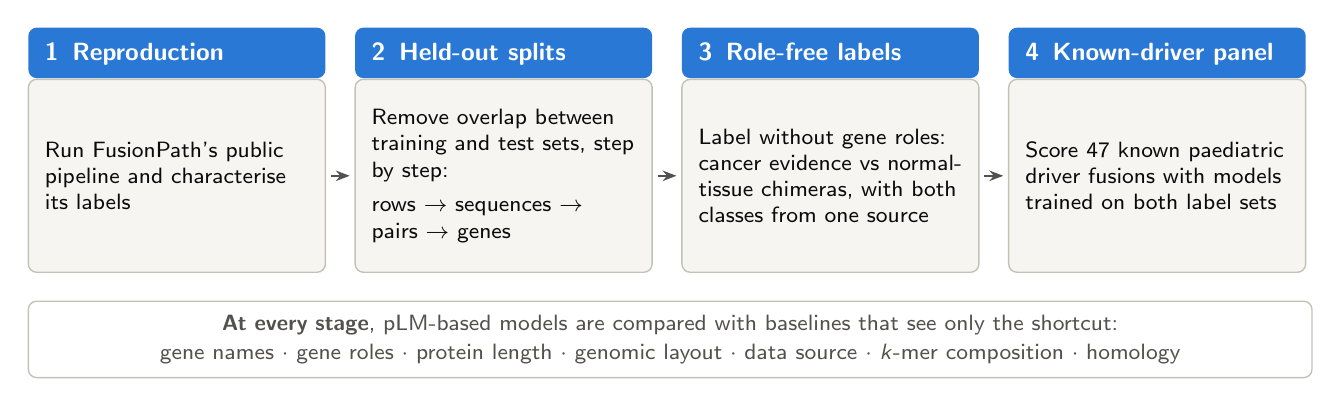
\begin{tikzpicture}[font=\footnotesize, text=ink]
  % stage bodies
  \node[stage] (s1) at (0,0)     {Run FusionPath's public pipeline and characterise its labels};
  \node[stage] (s2) at (4.15,0)  {Remove overlap between training and test sets, step by step:\\[3pt]
                                  rows $\rightarrow$ sequences $\rightarrow$ pairs $\rightarrow$ genes};
  \node[stage] (s3) at (8.3,0)   {Label without gene roles: cancer evidence vs normal-tissue chimeras,
                                  with both classes from one source};
  \node[stage] (s4) at (12.45,0) {Score 47 known paediatric driver fusions with models trained on both label sets};

  % stage headers
  \node[head] at (s1.north) {1\enspace Reproduction};
  \node[head] at (s2.north) {2\enspace Held-out splits};
  \node[head] at (s3.north) {3\enspace Role-free labels};
  \node[head] at (s4.north) {4\enspace Known-driver panel};

  % flow between stages
  \foreach \a/\b in {s1/s2, s2/s3, s3/s4}
    \draw[flow] ($(\a.east)+(0.06,0)$) -- ($(\b.west)+(-0.06,0)$);

  % baselines used at every stage
  \node[draw=edge, line width=0.5pt, rounded corners=3pt, inner sep=5pt, text width=15.95cm, align=center,
        below=0.35cm of s1.south west, anchor=north west, text=ink2]
    (base) {\textbf{At every stage}, pLM-based models are compared with baselines that see only the shortcut:\\[1pt]
            gene names $\cdot$ gene roles $\cdot$ protein length $\cdot$ genomic layout $\cdot$
            data source $\cdot$ \textit{k}-mer composition $\cdot$ homology};
\end{tikzpicture}
\end{document}
